\begin{figure*}[!htbp]
\begin{center}

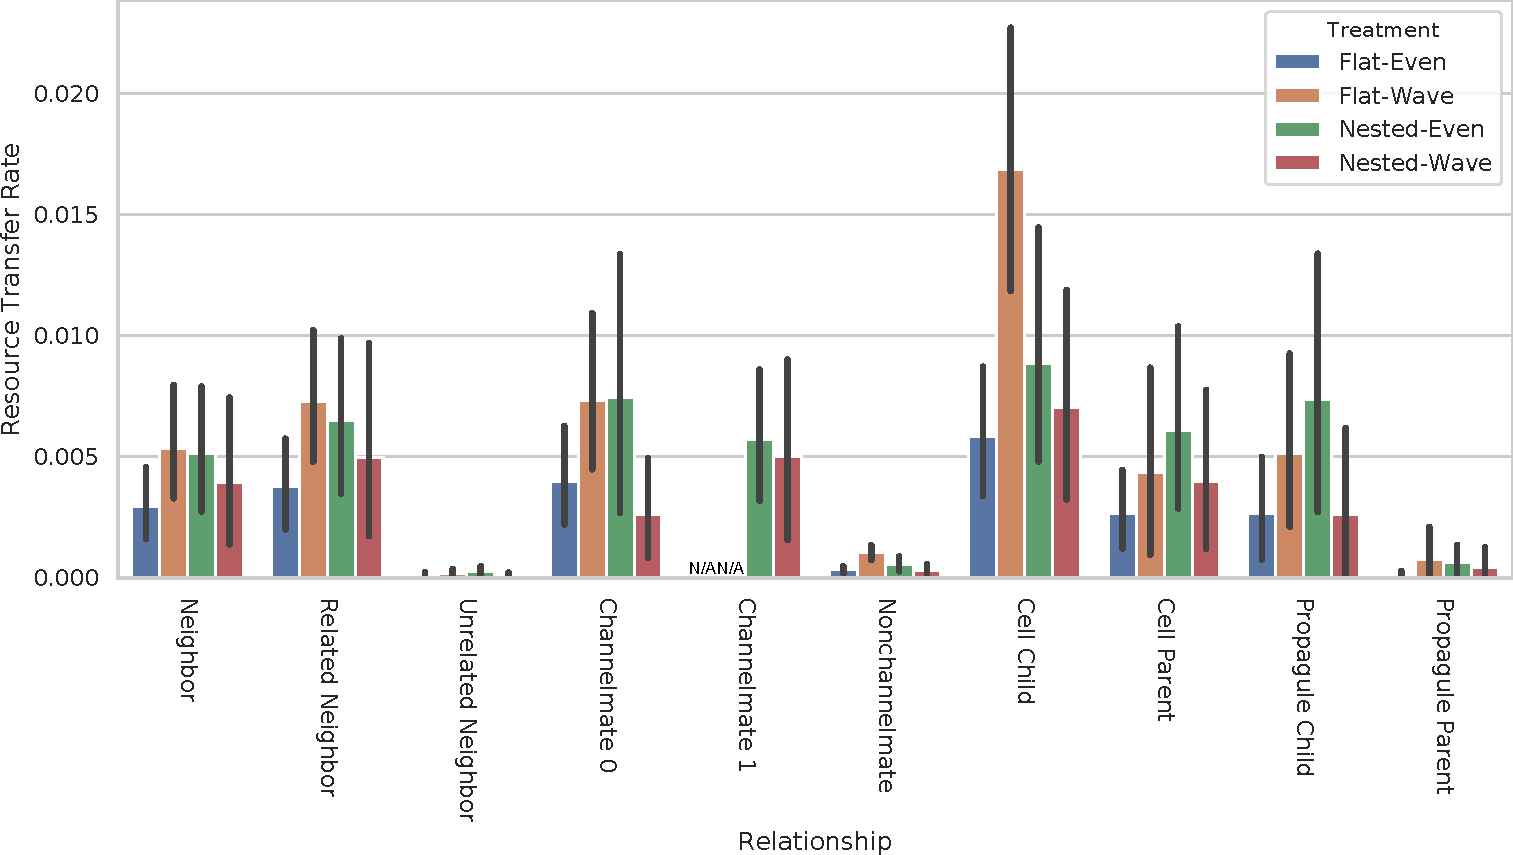
\includegraphics[width=\textwidth]{sharing/title=Resource_Transfer_Rate+_data_hathash_hash=ade957ec08284082+_script_fullcat_hash=e37b8d6f029c9f40+_source_hash=53a2252-clean+ext=}

\caption{
Resource sharing rates across donor-recipient relationships.
Neighbor describes any potential recipient cell.
Related neighbor describes a recipient cell that is a direct cellular progenitor or offspring of the donor, registered to a same hereditary group as the donor, or a member of a hereditary group that is a progenitor or offspring of the donor's.
Unrelated neighbors constitutes all other cells.
Channelmate refers to donor-recipient pairs that are registered to the same hereditary group.
Note that L1 groups are not defined in the flat treatment.
Non-channelmate recipients are not registered to any common hereditary groups with the potential donor.
Cell child and parent describe direct nuclear cell relationships between donor and recipient.
Finally, a propagule child relationship exists when a donor cell is a member of the apex-level hereditary group that directly begat the recipient cell's hereditary group.
A propagule parent relationship describes the reverse, when a recipient cell is a member of the apex-level hereditary group that directly begat the donor cell's hereditary group.
Error bars indicate 95\% confidence.
}
\label{fig:sharing}
\end{center}
\end{figure*}
